\section{DyNetKAT}
نک‌کت‌ پویا برای رفع برخی از کاستی‌های نت‌کت ارائه شده است
\cite{dynetkat}.
به صورت دقیق‌تر نت‌کت پویا، امکان توصیف به‌روز‌رسانی سیاست‌های شبکه و همچنین رفتار شبکه در مقابل چندین بسته را ممکن می‌سازد.

\subsection{سینتکس DyNetKAT}
در نت‌کت‌پویا، از رفتار انتها به انتها‌ی توصیف‌های شبکه در قالب عبارت‌های نت‌کت استفاده می‌شود.
به همین منظور سینتکس نت‌کت‌ پویا به صورت زیر تعریف می‌شود:
\begin{align*}
    N & :: = \mathrm{NetKAT}^{-dup}                    \\
    D & :: = \bot | N;D | x?N;D | x!N;D | D\parallel D
    D \oplus D | X                                     \\
      & X \triangleq D
\end{align*}
در سینتکس بالا
$\mathrm{NetKAT}^{-dup}$
قسمتی از زبان نت‌کت است که عبارت‌های
$dup$
از آن حذف شده است.
عبارت‌های
$dup$
در توصیف‌های نت‌کت تاثیری در رفتار یک عبارت ندارند و هدف از استفاده از آن‌ها ثبت یک اثر از هر بسته پس از پردازش توسط یکی از عناصر شبکه است و امکان استدلال بر روی رفتار شبکه را ممکن می‌سازد.
با توجه به این که در نت‌کت پویا رفتار انتها به انتهای یک عبارت نت‌کت مورد استفاده است، عبارت
$dup$
از سینتکس این زبان کنار گذاشته شده است.
نت‌کت‌پویا یک لیست از بسته‌های ورودی را پردازش می‌کند و یک لیست از مجموعه‌ی بسته‌های خروجی را تولید می‌کند.
اپراتور ترکیب متوالی
$N;D$
باعث می‌شود که یک بسته از لیست بسته‌های ورودی توسط سیاست
$N$
پردازش شود و سپس بسته‌ی توسط عبارت
$D$
پردازش می‌شود.
در نت‌کت پویا امکان ارتباط توسط عبارت‌هایی به شکل
$x!N$
و
$x?N$
توصیف می‌شوند که به ترتیب ارسال و دریافت یک عبارت نت‌کت را روی کانال
$x$
توصیف می‌کنند.
ترکیب موازی دو عبارت توسط
$D \parallel D$
توصیف می‌شود.
در نهایت رفتار‌های غیرقطعی توسط‌ عبارت‌هایی به شکل
$D \oplus D$
توصیف می‌شوند.

معنای عملیاتی نت‌کت پویا با استفاده از عبارت‌هایی به شکل
$(d,H,H')$
تعریف می‌شوند که
$d$
عبارت نت‌کت‌ پویا فعلی است،
$H$
لیست بسته‌هایی که در ادامه باید پردازش شوند
و
$H'$
لیست بسته‌هایی است که به صورت موفقیت‌آمیز توسط شبکه پردازش شده‌اند.
برچسب هر قانون که با
$\gamma$
مشخص می‌شود به صورت یکی از شکل‌های
$(\sigma,\sigma'),x!q,x?q$
یا
$rcfg(x,q)$
تعریف می‌شود.
\begin{align}
     & (cpol^{\checkmark}_{\_;})
    \frac{\sigma' \in \sem{p}(\sigma::\his{})}
    {(p;q,\sigma::H,H')\xrightarrow{(\sigma,\sigma')}
    (q,H,\sigma'::H') }                                     \\
     & (cpol_X)
    \frac{(p,H_0,H_1)\xrightarrow{\gamma}(p',H_0',H_1')}
    {(X,H_0,H_1)\xrightarrow{\gamma}(p',H_0',H_1')}
    X \triangleq p                                          \\
     & (cpol_{\_\oplus})
    \frac{(p,H_0,H_0')\xrightarrow{\gamma}(p',H_1,H_1')}
    {(p\oplus q,H_0,H_0')\xrightarrow{\gamma}(p',H_1,H_1')} \\
     & (cpol_{\oplus\_})
    \frac{(q,H_0,H_0')\xrightarrow{\gamma}(q',H_1,H_1')}
    {(p\oplus q,H_0,H_0')\xrightarrow{\gamma}(p',H_1,H_1')} \\
     & (cpol_{\_\parallel})
    \frac{(p,H_0,H_0')\xrightarrow{\gamma}(p',H_1,H_1')}
    {(p\parallel q,H_0,H_0')\xrightarrow{\gamma}(p' \parallel q,H_1,H_1')}
    \\
     & (cpol_{\parallel\_})
    \frac{(q,H_0,H_0')\xrightarrow{\gamma}(q',H_1,H_1')}
    {(p\parallel q,H_0,H_0')\xrightarrow{\gamma}(p \parallel q',H_1,H_1')}
    \\
     & (cpol_?)
    \frac{}
    {(x?p;q,H,H')\xrightarrow{x?p}(q,H,H')}
    \\
     & (cpol_!)
    \frac{}
    {(x!p;q,H,H')\xrightarrow{x!p}(q,H,H')}
    \\
     & (cpol_{!?})
    \frac{
        (q,H,H') \xrightarrow{x!p}(q',H,H')
        (s,H,H') \xrightarrow{x?p} (s',H,H')
    }{
        (q\parallel,H,H') \xrightarrow{rcfg(x,p)} (q'\parallel s',H,H')
    }                                                       \\
     & (cpol_{?!})
    \frac{
        (q,H,H') \xrightarrow{x?p}(q',H,H')
        (s,H,H') \xrightarrow{x!p} (s',H,H')
    }{
        (q\parallel,H,H') \xrightarrow{rcfg(x,p)} (q'\parallel s',H,H')
    }
\end{align}

\begin{figure}
    \centering
    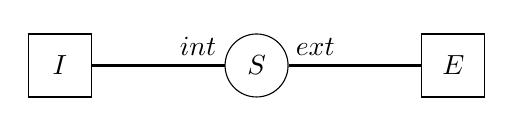
\begin{tikzpicture}[
            node distance={25mm},
            sw/.style = {draw, circle,minimum size=8mm},
            h/.style = {draw, rectangle,minimum size=8mm}
        ]
        \node[h] (i)  {$I$};
        \node[sw] (s) [right of=i]  {$S$};
        \node[h] (e)  [right of=s] {$E$};
        \draw [thick] (i)  -- node[above,pos=0.8]{$int$} (s);
        \draw [thick] (s) -- node[above,pos=0.2]{$ext$} (e);
    \end{tikzpicture}
    \caption{مثال دیوار آتش}
    \label{dynetkat:firewall}
\end{figure}

در ادامه چگونگی توصیف مثال دیوار آتش در شکل
\ref{dynetkat:firewall}
بیان می‌شود.
در این شبکه هدف این است که امکان ارتباط از داخل شبکه فراهم باشد ولی امکان ارسال بسته از خارج شبکه ممکن نباشد.
اما زمانی که یک بسته به خارج ارصال شد، دیوار آتش اجازه‌ی عبور بسته‌ها از بیرون را می‌دهد تا پاسخ بسته‌ها داده شود.
برای توصیف این شبکه می‌توان از عبارت نت‌کت پویای زیر استفاده کرد:
\begin{align*}
    Host  \triangleq   & secConReq!1;Host \oplus secConEnd!1;Host        \\
    Switch \triangleq  & (port = int) \cdot (port \la ext);Switch \oplus \\
                       & (port = ext)\cdot 0 ; Switch \oplus             \\
                       & secConReq?1;Switch'                             \\
    Switch' \triangleq & (port =int) \cdot (port \la ext);Switch' \oplus \\
                       & (port=ext)\cdot(port\la int);Switch' \oplus     \\
                       & secConEnd?1;Switch                              \\
    Init \triangleq    & Host \parallel Switch
\end{align*}
در این توصیف هاست امکان ارسال پیام برای شروع یا خاتمه‌ی یک ارتباط امن را دارد.
رفتار سوییچ در ابتدا به این صورت تعریف شده است که بسته‌ها را از پورت داخلی به پورت خارجی ارسال کند و تمام بسته‌هایی که از پورت خروجی وارد می‌شوند رها کند.
همچنین سوییچ امکان دریافت پیام شروع ارتباط امن را دارد.
پس از دریافت این پیام سوییچ اجازه می‌دهد تا بسته‌ها از پورت خروجی وارد شبکه شوند.
همچنین در صورتی که پیام خاتمه‌ی ارتباط امن را دریافت کند دوباره به رفتار اولیه‌ی خود بر می‌گردد.
در نهایت رفتار کل شبکه با استفاده از ترکیب موازی یک هاست و یک سوییچ در حالت اولیه توصیف می‌شود.
\begin{figure}[ht]
    \centerline{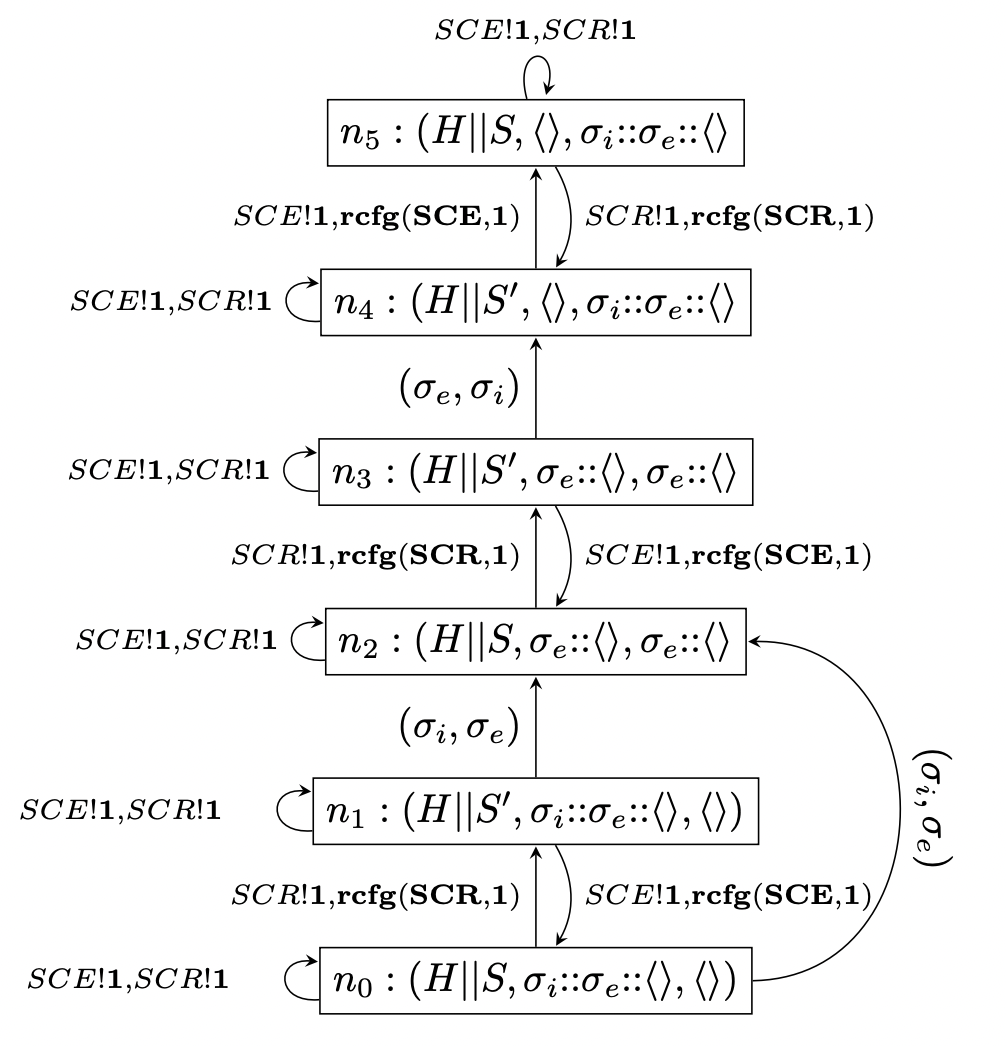
\includegraphics[width=0.8\textwidth]{mine/firewall-lts.png}}
    \caption{سیستم انتقال برچسب‌دار برای شبکه‌ی دیوار آتش}
    \label{firewall:lts}
\end{figure}
نمودار نمایش داده شده در شکل
\ref{firewall:lts}
سیستم انتقال این شبکه‌ را در حالتی که یک بسته روی پورت ورودی و یک بسته روی پورت خروجی شبکه وجود دارد نشان می‌دهد.
همانطور که در نمودار مشخص است، عملیات 
$(\sigma_e,\sigma_i)$
که به معنای ارسال بسته از پورت ورودی به پورت خروجی است تنها در قسمتی از این سیستم انتقال قابل دسترسی است که پیش از آن یکی از عملیات‌های 
$SCR?1$
یا
$rcfg(SCR,1)$
انجام شده باشند.
بنابراین در این حالت شبکه تنها در صورتی که بسته خارجی را به داخل ارسال می‌کند که پیش از آن پیام آغاز ارتباط امن دریافت کرده‌ باشد.

